% =====================================================================
%  NeuroVestigo -- ISBI 2027 four-page submission
%
%  Compressed from ../paper/main.tex (the full-length Cell Reports Methods
%  draft). Every number is copied from that file or from
%  ../ISBI2027_HANDOFF.md, and the table rows were checked against
%  benchmark/results/test/summary.csv. Nothing is re-derived.
%
%  Layout follows a 2026 ISBI four-pager (Goel et al., TrackletGPT,
%  arXiv:2601.13935): the data sit inside Methodology, followed by
%  Experiments and Results, Conclusion, Compliance with Ethical Standards,
%  Acknowledgments and References.
%
%  BUILD   tectonic main.tex   (or pdfLaTeX + BibTeX in Overleaf)
%          spconf.sty and IEEEbib.bst are the official ISBI template files
%          (biomedicalimaging.org, ISBI_template-master.zip).
%  LIMITS  ISBI 2027: single-blind. All technical content, including
%          figures and tables, within 4 pages. Page 5 ($200 fee) may hold
%          ONLY the ethics statement, acknowledgments and references.
%  OPEN    funding agencies and grant numbers (O.S.); author order (Prof.
%          Shefi).
% =====================================================================
\documentclass{article}
% T1 makes spconf's Times (ptm) resolve under XeTeX/tectonic too; without it
% XeTeX falls back to Latin Modern with no bold. Harmless under pdfLaTeX.
\usepackage[T1]{fontenc}
\usepackage{spconf,amsmath,amssymb,graphicx}
\usepackage{cite}
\usepackage{booktabs}
\usepackage{url}
\urlstyle{same}
\usepackage{xcolor}
\usepackage{tikz}
\usetikzlibrary{arrows.meta,positioning,calc,backgrounds,decorations.pathreplacing}
\usepackage{enumitem}
\setlist{nosep, leftmargin=12pt}
\graphicspath{{figures/}}

% figure palette (matches the PNG figures and ../paper/main.tex)
\definecolor{navy}{HTML}{16324F}
\definecolor{ourblue}{HTML}{1F6FB2}
\definecolor{teal}{HTML}{2CA6A4}
\definecolor{softgrey}{HTML}{E4E8ED}
\definecolor{midgrey}{HTML}{8B96A3}
\definecolor{amber}{HTML}{E1A93B}
\definecolor{crimson}{HTML}{C0392B}

% No extra gap between reference entries (spconf leaves LaTeX's default,
% stretched by \flushbottom); entries stay at 9 pt.
\makeatletter
\let\spconf@thebibliography\thebibliography
\def\thebibliography#1{\spconf@thebibliography{#1}%
  \setlength{\itemsep}{0pt}\setlength{\parsep}{0pt}}
\makeatother

% spconf's \@makecaption opens every caption with a 10 pt skip, meant to part
% a figure from the caption below it. A table's caption sits on top, where the
% skip only widens the gap above the table, so it is cancelled for tables.
\makeatletter
\def\nv@tabletype{table}
\let\nv@makecaption\@makecaption
\long\def\@makecaption#1#2{%
  \ifx\@captype\nv@tabletype\vskip-10pt\relax\fi
  \nv@makecaption{#1}{#2}}
\makeatother

% spconf sets \flushbottom, which spreads a column's spare space over its
% headings and float gaps (it opened a hole above Sec. 3.3); with ragged
% bottoms the spare space stays at the foot of the column instead.
\raggedbottom

% Gap between a two-column figure and the text below it (Fig. 1 opens page 2,
% Fig. 2 opens page 4): 14 pt instead of LaTeX's 20 pt.
\setlength{\dbltextfloatsep}{14pt plus 2pt minus 2pt}

\newcommand{\todo}[1]{\textcolor{red!80!black}{\textbf{[TODO: #1]}}}

\title{NeuroVestigo: topology-preserving segmentation and tracking of single
neurons in time-lapse microscopy}

% Author order to be confirmed with Prof. Shefi.
\name{Adi Oizerovich, Efrat Naomi Berkovich, Sharon Cohen, Ofek Ophir, Orit Shefi}
\address{Faculty of Engineering, Bar-Ilan University, Ramat Gan, Israel}

\begin{document}
\maketitle

% ---------------------------------------------------------------------
\begin{abstract}
Understanding neuronal growth and regeneration requires accurately quantifying single-cell morphology across multi-day, label-free recordings---a task still bottlenecked by labor-intensive manual tracing. Existing automated segmenters reliably resolve the soma but struggle with neurites and fail to preserve longitudinal instance identity. To address these limitations, we introduce NeuroVestigo, a parameter-efficient adaptation of the promptable video foundation model
SAM\,2 for time-lapse microscopy. Conditioned on a single annotated mask at frame~0, the model segments entire multi-day sequences. Utilizing dual-rank LoRA+, we train merely $13.9\,\%$ of the weights. The architecture is optimized via a connectivity-preserving objective that penalizes topological fractures. By backpropagating through an undetached temporal memory bank, we minimize longitudinal drift rather than merely measuring it. Evaluated on 12 held-out recordings from three splits, NeuroVestigo achieves state-of-the-art performance (cbDice $0.847 \pm 0.019$, IoU $0.751 \pm 0.024$), outperforming seven baselines across all metrics. Furthermore, it demonstrates markedly better temporal stability, exhibiting a minimal cbDice drift of $0.065$ between the first and final quartiles of the sequence, compared to $0.144$ for the most stable baselines. Code, weights, and a napari plug-in are available at \url{github.com/adioiz/NeuroVestigo} and \url{github.com/adioiz/neurons-labeling}.
\end{abstract}

\begin{keywords}
Neuron segmentation, cell tracking, phase-contrast microscopy,
topology-preserving loss, foundation models, live-cell imaging
\end{keywords}

% =====================================================================
\section{Introduction}
\label{sec:intro}

During development and regeneration, neurons dynamically extend, branch, and retract neurites to establish synaptic networks \cite{dotti1988polarity,lowery2009growthcone}. Neurite outgrowth is acutely modulated by chemical cues, such as axon guidance molecules \cite{lowery2009growthcone}, and by the physical microenvironment, including substrate topography, mechanical stiffness, and intercellular interactions \cite{shefi2005twophase,baranes2012topographic,marcus2017interactions}. Elucidating these processes necessitates precise, longitudinal quantification of single-neuron structural evolution---specifically neurite length, thickness, and branching topology \cite{odde1996stochastic}. Because neuronal growth is phasic \cite{shefi2005twophase,berkovich2025neurite}, capturing these kinematics requires dense frame-by-frame resolution, while high inter-cellular variance demands high-throughput analysis across large populations. We therefore employ label-free microscopy, enabling continuous multi-day imaging without the phototoxicity of fluorescent reporters. Yet, extracting morphometrics from this modality remains bottlenecked by labor-intensive manual tracing \cite{longair2011snt,berkovich2025neurite}, as automatically tracking a single neuron over time is still an unresolved challenge \cite{maska2023ctc}.

% Fig. 1 -- an ordinary [t] figure*: it appears at the top of the page after
% the one it is declared on. Declared here, after the first paragraph of the
% introduction (always on page 1), it opens page 2.
\begin{figure*}[t]
\centering
% Method overview for the ISBI 2027 version -- copied verbatim from
% paper/main.tex (Fig. 2 there, lines 772-797 and 801-945); edits are marked
% ISBI-EDIT. Panel (a) is paper/fig2_filmstrip.png, drawn by
% paper/make_filmstrip.py (A71_C1, its default), from
% benchmark/predictions/ours_23rec_topo (the released first-split model, which
% held that recording out).

% ----------------------------------------------------------
% Traced from real ground-truth masks -- training_data/masks/
% Sequence A71_C1, frames [0, 12, 24, 36, 48, 60, 72].  Generated by trace_masks.py;
% do not hand-edit.  Outlines are marching-squares contours of the
% annotated target; the skeleton is skimage.morphology.skeletonize.
% ----------------------------------------------------------
\newcommand{\neuronTight}{%
  \draw[mkfill] (-0.4418,-0.3361) -- (-0.4376,-0.2938) -- (-0.3826,-0.2642) -- (-0.3277,-0.2347) -- (-0.2621,-0.2156) -- (-0.2051,-0.1881) -- (-0.1649,-0.1438) -- (-0.1543,-0.1078) -- (-0.2135,-0.1332) -- (-0.2452,-0.1057) -- (-0.1818,-0.0846) -- (-0.1733,-0.0507) -- (-0.2262,-0.0190) -- (-0.2812,0.0106) -- (-0.3615,0.0148) -- (-0.4418,0.0106) -- (-0.4587,0.0486) -- (-0.3911,0.0486) -- (-0.3234,0.0486) -- (-0.2537,0.0338) -- (-0.1966,0.0063) -- (-0.1818,0.0676) -- (-0.1670,0.1374) -- (-0.1607,0.2072) -- (-0.1290,0.2051) -- (-0.1395,0.1311) -- (-0.1480,0.0550) -- (-0.1628,-0.0106) -- (-0.1205,-0.0528) -- (-0.0550,-0.0507) -- (0.0106,-0.0571) -- (0.0761,-0.0634) -- (0.1163,-0.0190) -- (0.1585,0.0233) -- (0.1628,0.0740) -- (0.1205,0.1163) -- (0.0972,0.1776) -- (0.0761,0.2410) -- (0.0507,0.3002) -- (0.0761,0.3129) -- (0.0994,0.2516) -- (0.1226,0.1903) -- (0.1522,0.1353) -- (0.1966,0.0951) -- (0.2558,0.0698) -- (0.3086,0.0381) -- (0.3573,0.0021) -- (0.4143,-0.0254) -- (0.4630,-0.0528) -- (0.4165,-0.0613) -- (0.3509,-0.0423) -- (0.3065,-0.0021) -- (0.2537,0.0296) -- (0.2072,-0.0042) -- (0.1881,-0.0698) -- (0.1374,-0.1036) -- (0.0698,-0.1205) -- (0.0063,-0.0994) -- (-0.0592,-0.0930) -- (-0.0972,-0.1395) -- (-0.0761,-0.2029) -- (-0.0592,-0.2706) -- (-0.0782,-0.2938) -- (-0.1036,-0.2347) -- (-0.1205,-0.1670) -- (-0.1607,-0.2114) -- (-0.1966,-0.2600) -- (-0.2516,-0.2473) -- (-0.3129,-0.2706) -- (-0.3657,-0.3023) -- (-0.4228,-0.3298);
}
\newcommand{\neuronTightSkel}{%
  \draw[mkskel] (-0.2347,-0.1226) -- (-0.2304,-0.1184) -- (-0.2262,-0.1184) -- (-0.2220,-0.1184) -- (-0.2177,-0.1184) -- (-0.2135,-0.1142) -- (-0.2093,-0.1099) -- (-0.2051,-0.1099) -- (-0.2008,-0.1099) -- (-0.1966,-0.1099) -- (-0.1924,-0.1057) -- (-0.1881,-0.1057) -- (-0.1839,-0.1015) -- (-0.1797,-0.0972) -- (-0.1755,-0.0972) -- (-0.1712,-0.0972) -- (-0.1670,-0.0972) -- (-0.1628,-0.0930) -- (-0.1585,-0.0930) -- (-0.1543,-0.0930) -- (-0.1501,-0.0930) -- (-0.1459,-0.0930) -- (-0.1416,-0.0930) -- (-0.1374,-0.0888) -- (-0.1332,-0.0846) -- (-0.1332,-0.0803) -- (-0.1332,-0.0761) -- (-0.1374,-0.0719) -- (-0.1374,-0.0676) -- (-0.1374,-0.0634) -- (-0.1416,-0.0592) -- (-0.1416,-0.0550) -- (-0.1459,-0.0507) -- (-0.1501,-0.0507) -- (-0.1543,-0.0465) -- (-0.1585,-0.0423) -- (-0.1628,-0.0381) -- (-0.1670,-0.0338) -- (-0.1712,-0.0296) -- (-0.1755,-0.0254) -- (-0.1755,-0.0211) -- (-0.1755,-0.0169) -- (-0.1797,-0.0127) -- (-0.1755,-0.0085) -- (-0.1755,-0.0042) -- (-0.1755,-0.0000) -- (-0.1755,0.0042) -- (-0.1755,0.0085) -- (-0.1755,0.0127) -- (-0.1755,0.0169) -- (-0.1712,0.0211) -- (-0.1712,0.0254) -- (-0.1712,0.0296) -- (-0.1712,0.0338) -- (-0.1712,0.0381) -- (-0.1712,0.0423) -- (-0.1670,0.0465) -- (-0.1670,0.0507) -- (-0.1670,0.0550) -- (-0.1670,0.0592) -- (-0.1670,0.0634) -- (-0.1628,0.0676) -- (-0.1628,0.0719) -- (-0.1628,0.0761) -- (-0.1628,0.0803) -- (-0.1628,0.0846) -- (-0.1628,0.0888) -- (-0.1628,0.0930) -- (-0.1628,0.0972) -- (-0.1628,0.1015) -- (-0.1628,0.1057) -- (-0.1585,0.1099) -- (-0.1585,0.1142) -- (-0.1585,0.1184) -- (-0.1585,0.1226) -- (-0.1543,0.1268) -- (-0.1543,0.1311) -- (-0.1543,0.1353) -- (-0.1501,0.1395) -- (-0.1501,0.1438) -- (-0.1501,0.1480) -- (-0.1501,0.1522) -- (-0.1501,0.1564) -- (-0.1501,0.1607) -- (-0.1459,0.1649) -- (-0.1459,0.1691) -- (-0.1459,0.1733) -- (-0.1459,0.1776) -- (-0.1459,0.1818) -- (-0.1459,0.1860) -- (-0.1459,0.1903) -- (-0.1459,0.1945) -- (-0.1459,0.1987) -- (-0.1459,0.2029) -- (-0.1459,0.2072) -- (-0.1459,0.2114) -- (-0.1459,0.2156);
  \draw[mkskel] (-0.1839,-0.0127) -- (-0.1881,-0.0127) -- (-0.1924,-0.0127) -- (-0.1966,-0.0085) -- (-0.2008,-0.0085) -- (-0.2051,-0.0085) -- (-0.2093,-0.0085) -- (-0.2135,-0.0042) -- (-0.2177,-0.0000) -- (-0.2220,-0.0000) -- (-0.2262,0.0042) -- (-0.2304,0.0042) -- (-0.2347,0.0085) -- (-0.2389,0.0085) -- (-0.2431,0.0127) -- (-0.2473,0.0127) -- (-0.2516,0.0169) -- (-0.2558,0.0211) -- (-0.2600,0.0211) -- (-0.2642,0.0211) -- (-0.2685,0.0254) -- (-0.2727,0.0254) -- (-0.2769,0.0254) -- (-0.2812,0.0296) -- (-0.2854,0.0296) -- (-0.2896,0.0296) -- (-0.2938,0.0296) -- (-0.2981,0.0296) -- (-0.3023,0.0296) -- (-0.3065,0.0296) -- (-0.3108,0.0338) -- (-0.3150,0.0338) -- (-0.3192,0.0338) -- (-0.3234,0.0338) -- (-0.3277,0.0338) -- (-0.3319,0.0338) -- (-0.3361,0.0338) -- (-0.3404,0.0338) -- (-0.3446,0.0338) -- (-0.3488,0.0338) -- (-0.3530,0.0338) -- (-0.3573,0.0338) -- (-0.3615,0.0338) -- (-0.3657,0.0338) -- (-0.3699,0.0338) -- (-0.3742,0.0338) -- (-0.3784,0.0296) -- (-0.3826,0.0296) -- (-0.3869,0.0296) -- (-0.3911,0.0296) -- (-0.3953,0.0296) -- (-0.3995,0.0296) -- (-0.4038,0.0296) -- (-0.4080,0.0296) -- (-0.4122,0.0296) -- (-0.4165,0.0296) -- (-0.4207,0.0296) -- (-0.4249,0.0296) -- (-0.4291,0.0296) -- (-0.4334,0.0296) -- (-0.4376,0.0296) -- (-0.4418,0.0296);
  \draw[mkskel] (-0.1290,-0.0846) -- (-0.1205,-0.0846) -- (-0.1120,-0.0846) -- (-0.1036,-0.0846) -- (-0.0951,-0.0803) -- (-0.0867,-0.0803) -- (-0.0782,-0.0761) -- (-0.0698,-0.0761) -- (-0.0613,-0.0719) -- (-0.0528,-0.0719) -- (-0.0444,-0.0676) -- (-0.0359,-0.0676) -- (-0.0275,-0.0676) -- (-0.0190,-0.0676) -- (-0.0106,-0.0719) -- (-0.0021,-0.0719) -- (0.0063,-0.0761) -- (0.0148,-0.0803) -- (0.0233,-0.0803) -- (0.0317,-0.0846) -- (0.0402,-0.0888) -- (0.0486,-0.0888) -- (0.0571,-0.0930) -- (0.0655,-0.0930) -- (0.0740,-0.0930) -- (0.0824,-0.0930) -- (0.0909,-0.0888) -- (0.0994,-0.0888) -- (0.1078,-0.0803) -- (0.1163,-0.0761) -- (0.1247,-0.0719) -- (0.1332,-0.0634) -- (0.1416,-0.0550) -- (0.1501,-0.0465) -- (0.1585,-0.0381) -- (0.1628,-0.0296) -- (0.1712,-0.0211) -- (0.1755,-0.0127) -- (0.1797,-0.0042) -- (0.1797,0.0042) -- (0.1881,0.0127) -- (0.1881,0.0211) -- (0.1881,0.0296) -- (0.1924,0.0381) -- (0.1966,0.0465) -- (0.1924,0.0550) -- (0.1924,0.0634) -- (0.1881,0.0719) -- (0.1839,0.0803) -- (0.1755,0.0888) -- (0.1670,0.0972) -- (0.1585,0.1057) -- (0.1501,0.1099) -- (0.1416,0.1184) -- (0.1332,0.1268) -- (0.1290,0.1353) -- (0.1247,0.1438) -- (0.1205,0.1522) -- (0.1163,0.1607) -- (0.1120,0.1691) -- (0.1120,0.1776) -- (0.1078,0.1860) -- (0.1036,0.1945) -- (0.1036,0.2029) -- (0.0994,0.2114) -- (0.0994,0.2199) -- (0.0951,0.2283) -- (0.0909,0.2368) -- (0.0867,0.2452) -- (0.0824,0.2537) -- (0.0782,0.2621) -- (0.0698,0.2706) -- (0.0655,0.2790) -- (0.0655,0.2875) -- (0.0655,0.2960) -- (0.0613,0.3044) -- (0.0655,0.3129) -- (0.0655,0.3213);
  \draw[mkskel] (0.2008,0.0507) -- (0.2051,0.0507) -- (0.2093,0.0507) -- (0.2135,0.0507) -- (0.2177,0.0507) -- (0.2220,0.0507) -- (0.2262,0.0507) -- (0.2304,0.0507) -- (0.2347,0.0507) -- (0.2389,0.0507) -- (0.2431,0.0507) -- (0.2473,0.0507) -- (0.2516,0.0507) -- (0.2558,0.0465) -- (0.2600,0.0465) -- (0.2642,0.0465) -- (0.2685,0.0423) -- (0.2727,0.0423) -- (0.2769,0.0423) -- (0.2812,0.0423) -- (0.2854,0.0381) -- (0.2896,0.0338) -- (0.2938,0.0296) -- (0.2981,0.0254) -- (0.3023,0.0254) -- (0.3065,0.0211) -- (0.3108,0.0169) -- (0.3150,0.0127) -- (0.3192,0.0085) -- (0.3234,0.0042) -- (0.3277,-0.0000) -- (0.3319,-0.0042) -- (0.3361,-0.0042) -- (0.3404,-0.0085) -- (0.3446,-0.0085) -- (0.3488,-0.0127) -- (0.3530,-0.0169) -- (0.3573,-0.0211) -- (0.3615,-0.0254) -- (0.3657,-0.0296) -- (0.3699,-0.0296) -- (0.3742,-0.0338) -- (0.3784,-0.0338) -- (0.3826,-0.0338) -- (0.3869,-0.0381) -- (0.3911,-0.0381) -- (0.3953,-0.0381) -- (0.3995,-0.0381) -- (0.4038,-0.0381) -- (0.4080,-0.0381) -- (0.4122,-0.0423) -- (0.4165,-0.0423) -- (0.4207,-0.0423) -- (0.4249,-0.0465) -- (0.4291,-0.0465) -- (0.4334,-0.0465) -- (0.4376,-0.0507) -- (0.4418,-0.0550) -- (0.4461,-0.0550) -- (0.4503,-0.0592) -- (0.4545,-0.0592);
  \draw[mkskel] (-0.1120,-0.0888) -- (-0.1120,-0.0930) -- (-0.1120,-0.0972) -- (-0.1163,-0.1015) -- (-0.1163,-0.1057) -- (-0.1163,-0.1099) -- (-0.1163,-0.1142) -- (-0.1163,-0.1184) -- (-0.1163,-0.1226) -- (-0.1163,-0.1268) -- (-0.1163,-0.1311) -- (-0.1205,-0.1353) -- (-0.1205,-0.1395) -- (-0.1205,-0.1438) -- (-0.1247,-0.1480) -- (-0.1290,-0.1480) -- (-0.1332,-0.1480) -- (-0.1374,-0.1522) -- (-0.1416,-0.1522) -- (-0.1459,-0.1564) -- (-0.1501,-0.1607) -- (-0.1501,-0.1649) -- (-0.1543,-0.1691) -- (-0.1585,-0.1733) -- (-0.1585,-0.1776) -- (-0.1628,-0.1818) -- (-0.1670,-0.1860) -- (-0.1712,-0.1903) -- (-0.1755,-0.1945) -- (-0.1797,-0.1987) -- (-0.1839,-0.2029) -- (-0.1881,-0.2072) -- (-0.1881,-0.2114) -- (-0.1924,-0.2156) -- (-0.1966,-0.2199) -- (-0.2008,-0.2199) -- (-0.2051,-0.2199) -- (-0.2093,-0.2199) -- (-0.2135,-0.2199) -- (-0.2177,-0.2199) -- (-0.2220,-0.2241) -- (-0.2262,-0.2241) -- (-0.2304,-0.2241) -- (-0.2347,-0.2241) -- (-0.2389,-0.2241) -- (-0.2431,-0.2241) -- (-0.2473,-0.2241) -- (-0.2516,-0.2283) -- (-0.2558,-0.2283) -- (-0.2600,-0.2283) -- (-0.2642,-0.2325) -- (-0.2685,-0.2325) -- (-0.2727,-0.2368) -- (-0.2769,-0.2368) -- (-0.2812,-0.2368) -- (-0.2854,-0.2410) -- (-0.2896,-0.2410) -- (-0.2938,-0.2410) -- (-0.2981,-0.2410) -- (-0.3023,-0.2452) -- (-0.3065,-0.2452) -- (-0.3108,-0.2495) -- (-0.3150,-0.2495) -- (-0.3192,-0.2537) -- (-0.3234,-0.2537) -- (-0.3277,-0.2579) -- (-0.3319,-0.2579) -- (-0.3361,-0.2621) -- (-0.3404,-0.2621) -- (-0.3446,-0.2664) -- (-0.3488,-0.2706) -- (-0.3530,-0.2706) -- (-0.3573,-0.2748) -- (-0.3615,-0.2748) -- (-0.3657,-0.2790) -- (-0.3699,-0.2833) -- (-0.3742,-0.2833) -- (-0.3784,-0.2875) -- (-0.3826,-0.2875) -- (-0.3869,-0.2875) -- (-0.3911,-0.2875) -- (-0.3953,-0.2917) -- (-0.3995,-0.2917) -- (-0.4038,-0.2917) -- (-0.4080,-0.2960) -- (-0.4122,-0.3002) -- (-0.4165,-0.3044) -- (-0.4207,-0.3044) -- (-0.4249,-0.3086) -- (-0.4291,-0.3129) -- (-0.4334,-0.3171) -- (-0.4376,-0.3213) -- (-0.4418,-0.3213) -- (-0.4461,-0.3256);
  \draw[mkskel] (-0.1205,-0.1480) -- (-0.1163,-0.1522) -- (-0.1120,-0.1564) -- (-0.1078,-0.1564) -- (-0.1036,-0.1607) -- (-0.1036,-0.1649) -- (-0.1036,-0.1691) -- (-0.1036,-0.1733) -- (-0.0994,-0.1776) -- (-0.0994,-0.1818) -- (-0.0994,-0.1860) -- (-0.0994,-0.1903) -- (-0.0951,-0.1945) -- (-0.0951,-0.1987) -- (-0.0951,-0.2029) -- (-0.0951,-0.2072) -- (-0.0909,-0.2114) -- (-0.0909,-0.2156) -- (-0.0909,-0.2199) -- (-0.0867,-0.2241) -- (-0.0867,-0.2283) -- (-0.0867,-0.2325) -- (-0.0824,-0.2368) -- (-0.0824,-0.2410) -- (-0.0824,-0.2452) -- (-0.0782,-0.2495) -- (-0.0782,-0.2537) -- (-0.0782,-0.2579) -- (-0.0782,-0.2621) -- (-0.0740,-0.2664) -- (-0.0740,-0.2706) -- (-0.0698,-0.2748) -- (-0.0698,-0.2790) -- (-0.0698,-0.2833) -- (-0.0655,-0.2875) -- (-0.0655,-0.2917) -- (-0.0613,-0.2960) -- (-0.0613,-0.3002) -- (-0.0613,-0.3044);
}
% skeleton 513 px vs 4977 mask px -> skeleton is 10.3\% of the mask

% framed panel holding a traced mask: #1 x, #2 y, #3 half-size, #4 macro
\newcommand{\maskpanel}[4]{%
  \begin{scope}[shift={(#1,#2)}]
    \draw[black!35, line width=0.35pt, fill=white] (-#3,-#3) rectangle (#3,#3);
    \begin{scope}[scale={2*#3}]#4\end{scope}
  \end{scope}
}

\begin{tikzpicture}[
  font=\small,
  rule/.style={draw=black!45, line width=0.4pt},
  plab/.style={font=\bfseries\small, text=black, anchor=north west},
  ptit/.style={font=\small, text=black, anchor=north west},
  note/.style={font=\scriptsize, text=black!60, align=left},
  sm/.style={font=\fontsize{6.4}{7.4}\selectfont, text=black!60},
  bx/.style={rounded corners=1pt, align=center, inner sep=2.5pt,
             line width=0.5pt, font=\fontsize{7}{8}\selectfont},
  frz/.style={bx, fill=black!5,    draw=black!45},
  lra/.style={bx, fill=ourblue!10, draw=ourblue!75},
  trn/.style={bx, fill=teal!10,    draw=teal!75},
  ar/.style={-{Stealth[length=1.7mm,width=1.4mm]}, draw=black!65, line width=0.5pt},
  loop/.style={-{Stealth[length=1.7mm,width=1.4mm]}, draw=amber!85!black,
               line width=0.7pt},
  grad/.style={-{Stealth[length=1.7mm,width=1.4mm]}, draw=crimson!85,
               line width=0.6pt},
  mkfill/.style={fill=mk!25, draw=mk!90!black, line width=0.25pt},
  mkskel/.style={draw=mk2, line width=0.4pt, line cap=round},
  nd/.style={circle, draw=black!60, fill=white, line width=0.5pt,
             minimum size=0.26cm, inner sep=0pt},
]

% ==================  (a)  the propagation task  ==================
\node[plab] at (0.00,7.55) {(a)};
\node[ptit] at (0.62,7.55)
     {One annotation at $t=0$ propagates through the whole recording};

% Real phase contrast: the frame-0 ground-truth prompt (navy) and the model's
% own propagated masks (teal).  Seven 1.24 cm cells on a 2.30 cm pitch, 50 um
% scale bar burnt into the last cell.  Built by make_filmstrip.py, which
% refuses to draw a recording the model trained on, and refuses to draw at all
% unless the stack re-scores to the IoU in results/test/ours_23rec_topo.csv.
\node[anchor=south west, inner sep=0] at (0.53,5.80)
     {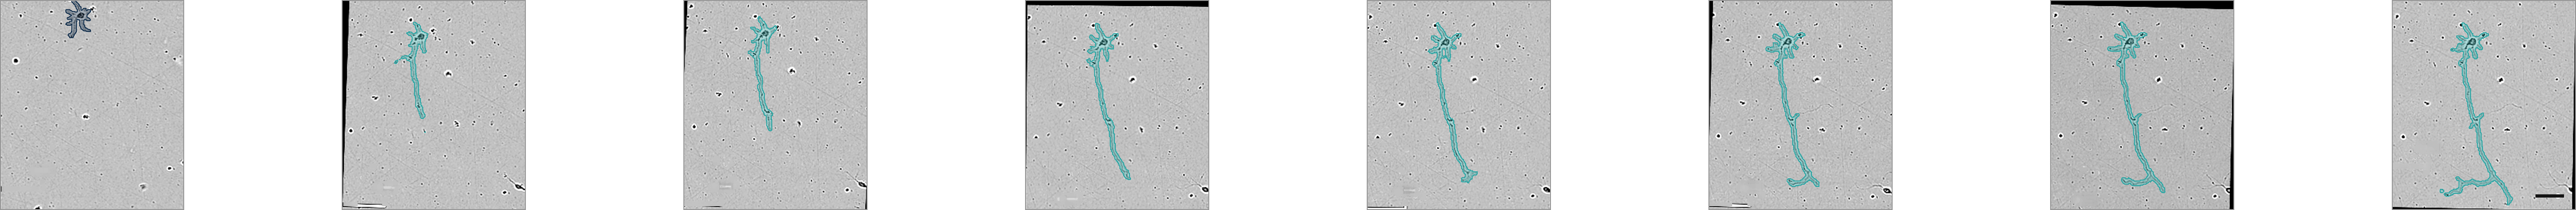
\includegraphics[width=15.04cm]{fig2_filmstrip}};

\draw[rule] (0.90,5.70) -- (15.35,5.70);
\foreach \x in {1.15,3.45,5.75,8.05,10.35,12.65,14.95}
  \draw[rule] (\x,5.70) -- (\x,5.60);
\foreach \x/\lb in {1.15/0, 3.45/12, 5.75/24, 8.05/36, 10.35/48, 12.65/60,
                    14.95/72}
  \node[sm, anchor=north] at (\x,5.56) {\lb};
\node[sm, anchor=west] at (15.45,5.64) {h};
\node[sm, text=navy, anchor=north] at (1.15,5.26) {given};
\node[sm, anchor=north east] at (16.20,5.26) {scale bar $50\,\mu$m};
\node[sm, anchor=north] at (9.20,5.26)
     {propagated with no further prompt, correction or re-initialization};

\draw[rule] (0,4.88) -- (16.20,4.88);

% ==================  (b)  where the model is adapted  ============
\node[plab] at (0.00,4.68) {(b)};
\node[ptit] at (0.62,4.68) {Adaptation sites};
\node[note, anchor=north west] at (0.62,4.32)
     {$5{,}557{,}250$ of $39{,}876{,}930$ parameters trainable ($13.9\,\%$)};

\node[frz, minimum width=2.30cm, minimum height=0.74cm, anchor=west] (enc)
     at (0.10,3.35) {Image encoder\\{\fontsize{6}{7}\selectfont Hiera-tiny}};
\node[lra, minimum width=1.70cm, minimum height=0.74cm, anchor=west] (hier)
     at (2.85,3.35) {blocks 10--11\\{\fontsize{6}{7}\selectfont $r{=}8$}};
\node[trn, minimum width=2.10cm, minimum height=0.74cm, anchor=west] (pe)
     at (6.10,3.35) {Prompt encoder\\{\fontsize{6}{7}\selectfont frame-0 mask}};

\node[lra, minimum width=2.55cm, minimum height=0.80cm, anchor=west] (mem)
     at (0.10,1.95) {Memory attention\\{\fontsize{6}{7}\selectfont $r{=}16$,
       40 sites}};
\node[lra, minimum width=2.55cm, minimum height=0.80cm, anchor=west] (dec)
     at (3.30,1.95) {Mask decoder\\{\fontsize{6}{7}\selectfont $r{=}16$,
       28 sites}};
\node[trn, minimum width=2.90cm, minimum height=0.50cm, anchor=west] (menc)
     at (2.00,0.72) {Memory encoder $+$ bank};

\draw[ar] (enc.east) -- (hier.west);
\draw[ar] (hier.south) -- ++(0,-0.26) -| (mem.north);
\draw[ar] (mem.east) -- (dec.west);
\draw[ar] (pe.south) -- ++(0,-0.42) -| ([xshift=8mm]dec.north);
\draw[ar] (dec.east) -- ++(0.24,0) node[right, sm, text=black] {$\hat{m}_t$};
\draw[loop] (dec.south) -- (dec.south |- menc.north);
\draw[loop] (menc.west) -| (mem.south);
\node[sm, text=amber!55!black, anchor=west] at (0.10,0.18)
     {the bank read at $t$ holds the mask predicted at $t-1$};

% --- key
\begin{scope}[shift={(0.10,-0.30)}]
  \node[frz, minimum width=0.26cm, minimum height=0.17cm, anchor=west] at (0,0) {};
  \node[sm, anchor=west, text=black] at (0.32,0) {frozen};
  \node[lra, minimum width=0.26cm, minimum height=0.17cm, anchor=west] at (1.25,0) {};
  \node[sm, anchor=west, text=black] at (1.57,0) {LoRA-adapted, $0.91$\,M};
  \node[trn, minimum width=0.26cm, minimum height=0.17cm, anchor=west] at (4.45,0) {};
  \node[sm, anchor=west, text=black] at (4.77,0) {trained directly, $4.64$\,M};
\end{scope}

% ==================  (c)  the objective  =========================
\draw[rule] (9.10,4.68) -- (9.10,-0.50);

\node[plab] at (9.35,4.68) {(c)};
\node[ptit] at (9.97,4.68) {Objective};
\node[note, anchor=north west] at (9.97,4.32)
     {16-frame clips, bank not detached};

\node[sm, anchor=south] at (12.40,3.58) {memory writes};
\node[nd] (n0) at (10.15,3.42) {};
\node[nd] (n1) at (11.35,3.42) {};
\node[nd] (n2) at (12.55,3.42) {};
\node[nd] (n3) at (14.75,3.42) {};
\node[sm] at (13.65,3.42) {$\cdots$};
\draw[ar] (n0) -- (n1);
\draw[ar] (n1) -- (n2);
\draw[ar] (n2) -- (13.30,3.42);
\draw[ar] (14.00,3.42) -- (n3);
\foreach \x/\lb in {10.15/t, 11.35/{t{+}1}, 12.55/{t{+}2}, 14.75/{t{+}15}}
  \node[sm, anchor=north] at (\x,3.18) {$\lb$};

\draw[grad] (14.75,2.92) .. controls (13.80,2.46) and (11.10,2.46) .. (10.15,2.92);
\node[sm, text=crimson!85, anchor=north] at (12.45,2.50)
     {gradient retained back to the start of the clip};

% --- the composite loss, as a ruled table
\draw[rule] (9.35,2.02) -- (16.20,2.02);
\node[sm, anchor=west] at (9.42,1.86) {weight};
\node[sm, anchor=west] at (10.42,1.86) {term};
\node[sm, anchor=west] at (12.30,1.86) {compares};
\draw[rule] (9.35,1.72) -- (16.20,1.72);
\foreach \y/\w/\t/\c in {1.52/{$3.0$}/{Focal}/{pixels},
                         1.22/{$2.0$}/{Dice}/{regions}}{
  \node[font=\fontsize{6.8}{7.8}\selectfont, anchor=west] at (9.42,\y) {\w};
  \node[font=\fontsize{6.8}{7.8}\selectfont, anchor=west] at (10.42,\y) {\t};
  \node[sm, anchor=west] at (12.30,\y) {\c};
}
\foreach \y/\w/\t/\c in {0.92/{$0.3$}/{cbDice}/{centerlines},
                         0.62/{$0.3$}/{Supervoxel}/{connected components}}{
  \node[font=\fontsize{6.8}{7.8}\selectfont, text=ourblue, anchor=west] at (9.42,\y) {\w};
  \node[font=\fontsize{6.8}{7.8}\selectfont, text=ourblue, anchor=west] at (10.42,\y) {\t};
  \node[sm, text=ourblue!85!black, anchor=west] at (12.30,\y) {\c};
}
\draw[rule] (9.35,0.44) -- (16.20,0.44);

% --- what the two topology terms actually look at
\colorlet{mk}{black!45}\colorlet{mk2}{ourblue}
\maskpanel{9.78}{-0.06}{0.36}{\neuronTight\neuronTightSkel}
% ISBI-EDIT: the long paper's note ("a severed branch is invisible to an area
% term and costly to a centerline term") is dropped -- paper/main.tex records
% (Discussion, caution b) that cbDice tracks IoU to within 0.02 when branches
% are deleted, so the sensitivity claim has no measurement behind it. What is
% kept is measured: skeleton 513 px vs 4977 mask px on this frame.
\node[sm, anchor=west, align=left] at (10.30,-0.06)
     {held-out target, skeleton in blue:\\
      cbDice weights thin branches; the supervoxel\\
      term catches cuts and bridges};

\end{tikzpicture}

\caption{\textbf{Method.} \textbf{(a)}~A single ground-truth mask at frame~0 (navy) is propagated through recording \texttt{A71\_C1} without subsequent prompting (teal, model predictions). \textbf{(b)}~Adaptation sites. \textbf{(c)}~The memory bank remains undetached from the computation graph across 16-frame sequences; two topology-preserving terms augment the Focal and Dice objectives (Eq.~\ref{eq:loss}).}
\label{fig:method}
\end{figure*}

Three intrinsic properties render this task uniquely challenging. First, neurites are only a few pixels wide; consequently, minimal pixel misclassifications can induce catastrophic topological fractures that incur negligible penalties under standard area-based metrics. Second, label-free imaging suffers from inherently low signal-to-noise ratios. Finally, the target undergoes continuous morphological expansion amid identical distractors, mandating strict disambiguation and the longitudinal preservation of identity.

Current computational frameworks address this challenge only partially. Standard cell segmenters (e.g., Cellpose-SAM \cite{pachitariu2025cellposesam} and Omnipose \cite{cutler2022omnipose}) and domain-specific models such as NeuroQuantify \cite{dang2024neuroquantify} process frames independently, failing to preserve longitudinal instance identity. Post hoc temporal linking \cite{maska2023ctc,gallusser2024trackastra} cannot repair topological fractures introduced during segmentation, while tracking pipelines such as NeuriteTracker \cite{fusco2016neuritetracker} require fluorescent labels. Promptable models, by contrast, let the user select a single target: SAM\,2 \cite{ravi2025sam2} and SAM\,3 \cite{carion2025sam3} propagate a spatial prompt through a memory bank, and $\mu$SAM \cite{archit2025microsam} adapts SAM \cite{kirillov2023sam} specifically for microscopy. Crucially, none of these architectures are optimized to maintain the structural connectivity of ultra-fine, pixel-scale branches. Although topology-aware loss formulations \cite{shit2021cldice,shi2024cbdice,grim2025supervoxel} are explicitly designed to penalize such disconnections, they remain, to our knowledge, unintegrated within the optimization of promptable video models.

To address this, we introduce \textbf{NeuroVestigo}, a SAM\,2.1 adaptation employing dual-rank LoRA+, optimized via backpropagation through an undetached memory bank to prioritize longitudinal propagation over per-frame segmentation. Furthermore, we propose a topology-preserving objective that integrates cbDice and supervoxel loss with conventional Focal and Dice terms, and rigorously select checkpoints via Betti-0 error minimization. Finally, we provide comprehensive benchmarking, including temporal degradation analysis---and publicly release our code, weights, and annotation plug-in.

% =====================================================================
\section{Methodology}
\label{sec:method}

\subsection{Data and annotation}
\label{sec:data}

Primary cortical neurons from P0--P1 BALB/c mice
\cite{berkovich2025neurite} were imaged label-free on an IncuCyte SX5
(Sartorius) with a $10\times$ objective, one frame per hour. Each of the 32 recordings is a crop
centered on one target neuron, 148--615 by 146--498\,px, with 57--97 frames (most often 73); 2{,}490 masks were
annotated in total. The target covers $2.485\,\%$ of a frame on
average and as little as $0.217\,\%$. We train three models on 23/5/4 train/val/test splits with a shared validation set and disjoint test sets. Masks were drawn in \texttt{neurons-labeling}, a napari
plug-in built for this work: a neuron is painted on frame~0 and propagated,
any frame can be corrected, and propagation is re-run from there. Every mask was hand-edited.

\subsection{Promptable propagation}
\label{sec:prop}

We adapt SAM\,2.1 with the Hiera-tiny image encoder
\cite{ravi2025sam2,ryali2023hiera}. SAM\,2 is prompted geometrically on one
frame, and a memory bank carries the prompt forward. With $I_t$ the frame at
time $t$, $E$ the encoder and $M_t$ the bank after frame $t$ (frame~0 plus the six most recent frames),
\begin{equation}
\begin{split}
F_t &= \mathrm{MemAttn}\big(E(I_t),\, M_{t-1}\big),\qquad
\hat{m}_t = \mathrm{Dec}(F_t),\\
M_t &= \big[M_{t-1};\; \mathrm{MemEnc}(I_t, \hat{m}_t)\big],
\end{split}
\label{eq:recurrence}
\end{equation}
with $M_0$ formed from the ground-truth mask of frame~0. During step $t$, the memory bank integrates the mask predicted at $t-1$,
ensuring each prediction is recursively conditioned on all preceding outputs.
Consequently, the frame-level loss propagates gradients to the adapters
through every prior memory write back to the clip's origin---strictly
requiring that the memory bank remains undetached from the computation graph
(Fig.~\ref{fig:method}c). The memory-attention adapters and memory encoder,
which dictate cross-frame dynamics, receive optimization signals exclusively
along these temporal trajectories. Detaching the graph would degenerate the
objective into independent spatial segmentation, failing to optimize
longitudinal mask propagation. We therefore optimize via backpropagation
through time across 16-frame sequences, with each conditioned purely on its
initial frame.

Frames are resized to $1024\times1024$ (nearest-neighbor for masks). During
inference, the entire sequence is propagated continuously without
supplementary prompting, manual correction, or re-initialization. Output
logits are strictly zero-thresholded and rescaled to the native spatial
resolution.

\subsection{Parameter-efficient adaptation}
\label{sec:lora}

We employ LoRA \cite{hu2022lora} with the LoRA+ \cite{hayou2024loraplus} optimal learning rate ratio ($\lambda=16$; $10^{-4}$ and $1.6\times10^{-3}$ for the two low-rank factors), maintaining a scaling constant of $\alpha/r=2$ across all sites. Adapters are injected at 76 projections (Fig.~\ref{fig:method}b): 40 in memory attention and 28 in the mask decoder ($r=16$, $\alpha=32$), alongside 8 in Hiera blocks 10--11 ($r=8$, $\alpha=16$); the encoder's 27.2\,M pretrained weights stay frozen. The prompt encoder, memory encoder, object-pointer embeddings, and decoder MLP heads are trained directly without a low-rank constraint at a learning rate of $10^{-5}$. In total, $5{,}557{,}250$ of $39{,}876{,}930$ parameters are trainable: $0.91$\,M in the adapters and $4.64$\,M in these full-rank modules.

\subsection{Topology-preserving loss}
\label{sec:loss}

The predicted mask is supervised by
\begin{equation}
\mathcal{L} = 3\,\mathcal{L}_{\text{focal}} + 2\,\mathcal{L}_{\text{Dice}}
 + 0.3\,\mathcal{L}_{\text{cbDice}} + 0.3\,\mathcal{L}_{\text{sv}} .
\label{eq:loss}
\end{equation}

Focal \cite{lin2017focal} ($\gamma=2$, $\alpha=0.25$) and Dice \cite{milletari2016vnet} terms comprise the original SAM\,2 mask supervision, with Focal loss preventing the overwhelming background from dominating. Because severed or fused branches alter negligible pixel volumes, both terms remain insensitive to topological fractures. Therefore, cbDice \cite{shi2024cbdice} extends clDice \cite{shit2021cldice} by comparing prediction and target skeletons, down-weighting thick regions by their local radius so the soma cannot dominate thin branches.

The supervoxel loss \cite{grim2025supervoxel} locates the pixels responsible
for a topological error. The prediction is thresholded at $0.5$, and its
false-negative and false-positive masks are decomposed into 4-connected
components, ensuring that diagonal adjacencies do not confer structural continuity. A
false-negative component adjoining two or more predicted components is a bridge the model failed to predict, thereby inducing a topological \emph{split}; conversely, a false-positive component whose removal disconnects the prediction is a bridge it invented and causes a \emph{merge}. Defining
$\mathcal{N}$ and $\mathcal{P}$ as the unions of split- and merge-causing components, $\Omega$ as the spatial domain of the frame, and $\bar{\mathcal{L}}_0$ as a spatially averaged binary cross-entropy,
\begin{equation}
\mathcal{L}_{\text{sv}} =
 \tfrac12\,\bar{\mathcal{L}}_0\big(\Omega\setminus(\mathcal{N}\cup\mathcal{P})\big)
 + \tfrac14\,\bar{\mathcal{L}}_0(\mathcal{N})
 + \tfrac14\,\bar{\mathcal{L}}_0(\mathcal{P}).
\label{eq:sv}
\end{equation}
Each term is averaged over its own pixels, so a two-pixel bridge carries a quarter of the term. Both topology terms are evaluated at $512 \times 512$, with the supervoxel term's critical masks upsampled so it is computed at full resolution; resampling below the native dimensions would obliterate the 1--2-pixel processes these terms explicitly protect.

\subsection{Training and model selection}
\label{sec:train}

We optimize using AdamW \cite{loshchilov2019adamw} (weight decay $0.05$) for 110 epochs on 16-frame sequences with temporal stride 4. We employ a batch size of two clips, a two-epoch warmup, cosine decay to $5\,\%$ of the peak learning rate, and gradient-norm clipping at $1.0$. Training runs in bfloat16 on one NVIDIA B200 (${\approx}23$\,h). Spatial and photometric augmentations---flips, rotation ($\pm25^{\circ}$), shear ($\pm20^{\circ}$), and brightness/contrast ($\pm15\,\%$)---are applied identically across all frames within a sequence. Model selection uses the validation split: among checkpoints within $0.005$ validation IoU of the maximum, we select the epoch minimizing raw validation Betti-0 error (absolute difference between predicted and ground-truth connected components). No temporal smoothing is applied.
% =====================================================================
\section{Experiments and Results}
\label{sec:results}

% Fig. 2 -- an ordinary [t] figure*, declared at the start of Sec. 3, which is
% typeset on page 3, so it opens page 4.
\begin{figure*}[t]
\centering
% Drawn by make_fig_qual.py (benchmark/make_proof_panel.py, relabeled for a
% two-column page); predictions from benchmark/predictions/ours_23rec_topo.
\includegraphics[width=\textwidth]{proof_A71_C1_isbi}
\caption{\textbf{Qualitative comparison} on held-out recording
\texttt{A71\_C1} at frames 8 and 62; per-panel IoU inset.}
\label{fig:qual}
\end{figure*}

\subsection{Protocol and baselines}
\label{sec:protocol}

Since frame~0 is the prompt, it is not scored, leaving 328 evaluated test frames per split. Metrics are computed per frame on native-resolution hard masks, averaged per recording, and then across recordings with equal weight. We report IoU, Dice, cbDice and clDice; because clDice is never optimized during training, it independently validates cbDice. Zero-shot SAM\,2 and SAM\,3 \cite{carion2025sam3} receive the frame\nobreakdash-0 mask; $\mu$SAM \cite{archit2025microsam} receives a ground-truth box, padded by 6\,px, on every frame. Automatic baselines---Cellpose-SAM \cite{pachitariu2025cellposesam}, Omnipose \cite{cutler2022omnipose}, and NeuroQuantify \cite{dang2024neuroquantify}---operate at $\times2$, $\times3$, and $\times4$ input scales, respectively. SAM\,3.1 uses the text prompt \emph{cells}. Finally, automatic methods receive an oracle reduction to the target: the union of all predicted regions overlapping it.
Hyperparameters and backbones were tuned solely on the validation split.
% Model variants, dropped from the text 2026-10-05 (all in the repository's
% benchmark scripts): muSAM vit_l_lm (vit_b_lm 0.42 vs 0.56 validation IoU);
% Omnipose bact_phase_omni (cyto2_omni detects nothing on validation).

\subsection{Benchmarking against existing methods}
\label{sec:res:benchmark}

NeuroVestigo outperforms every baseline across all metrics (Table~\ref{tab:main}) and on IoU in at least 11 of the 12 test recordings. Because zero-shot SAM\,2 shares the same backbone and prompt, the resulting gains ($0.143$ IoU, $0.127$ cbDice) stem from our fine-tuning. On clDice, our independent topological check, the improvement reaches $0.136$. A larger backbone fails to close this gap: identically prompted zero-shot SAM\,3 performs within the noise of zero-shot SAM\,2 ($0.620$ vs.\ $0.609$ IoU).

% Table 1 -- [!h], between the two paragraphs of Sec. 3.2: printed here, or
% at the top of the next column if it does not fit there.
\begin{table}[!h]
\centering
\caption{\textbf{Test set results.} Mean\,$\pm$\,SD over three repeated hold-out splits (328 test frames each, frame~0 excluded); $t$ denotes frame index.}
\label{tab:main}
\vspace{2pt}
\scriptsize
\setlength{\tabcolsep}{2pt}
\begin{tabular}{@{}llcccc@{}}
\toprule
Method & Prompt & IoU & Dice & \textbf{cbDice} & clDice \\
\midrule
\textbf{NeuroVestigo}  & mask, $t{=}0$      & \textbf{.751}$\pm$.024 & \textbf{.856}$\pm$.016 & \textbf{.847}$\pm$.019 & \textbf{.941}$\pm$.019 \\
SAM\,2 (zero-shot)     & mask, $t{=}0$      & .609$\pm$.050 & .743$\pm$.046 & .720$\pm$.063 & .805$\pm$.066 \\
SAM\,3 (mask)          & mask, $t{=}0$      & .620$\pm$.010 & .745$\pm$.002 & .747$\pm$.014 & .797$\pm$.013 \\
$\mu$SAM (box)         & GT box, all $t$    & .623$\pm$.049 & .761$\pm$.039 & .822$\pm$.041 & .885$\pm$.046 \\
Cellpose-SAM           & none               & .519$\pm$.072 & .648$\pm$.083 & .658$\pm$.088 & .715$\pm$.098 \\
NeuroQuantify          & none               & .358$\pm$.137 & .475$\pm$.167 & .497$\pm$.174 & .547$\pm$.201 \\
Omnipose               & none               & .289$\pm$.026 & .440$\pm$.031 & .571$\pm$.035 & .648$\pm$.040 \\
SAM\,3.1 (text)        & none               & .176$\pm$.038 & .239$\pm$.058 & .246$\pm$.059 & .263$\pm$.062 \\
\bottomrule
\end{tabular}
\end{table}

A single frame\nobreakdash-0 mask is more informative than a ground-truth box on every frame: NeuroVestigo leads $\mu$SAM, the strongest baseline on cbDice, by $0.128$ IoU and $0.025$ cbDice, the latter within noise. A bounding box is a weak prompt for a branched cell, which fills only $19\,\%$ of its bounding area on average. Masks stay nearly whole, as the supervoxel term and Betti-0 selection intend: predictions average $1.42$ connected components per frame against $1.04$ in the ground truth. Achieving peak clDice simultaneously confirms this low count does not stem from dropped branches. As the arbor grows (Fig.~\ref{fig:qual}), NeuroVestigo successfully tracks the thin distal branches that baselines partially miss (green).
% Sources (all test set, Table 1 protocol). clDice gain over SAM 2: 0.9466 -
% 0.8305 = 0.116 (summary.csv). SAM 3 vs SAM 2 zero-shot, IoU per recording
% (A71, A81, A12_C3, A12_C1): .760/.760, .736/.644, .347/.593, .668/.561 ->
% sign changes, hence "within noise". Box fill and worst frame re-checked
% 2026-10-03 on the stored predictions: target fills 21.2% of its bounding box
% (recording-weighted; 29.3% in Q1, 14.1% in Q4); lowest per-frame IoU ours
% 0.581, SAM 2 0.277 (6 frames < 0.3), every other baseline lower.
% "Nearly whole ... intend", not "validating": no run without the supervoxel
% term exists (every checkpoint config has use_supervoxel=True, weight 0.3), and
% the Betti-0 tie-break barely moves the count on test. Released vs IoU-best
% epoch of the same run (ours_23rec), checked 2026-10-03: 1.36 vs 1.39
% pieces/frame, Betti-0 error 0.365 vs 0.390, one piece in 79% vs 78% of
% frames; per recording .10/.19, 1.07/1.12, .10/.08, .20/.16 -> sign changes,
% within noise. Zero-shot SAM 2: 1.44 pieces, 76% one piece. A81_C1 averages
% 2.08 pieces/frame for the released model.
% Components per frame, other methods (kept out of the text by decision):
% Cellpose-SAM 3.25, NeuroQuantify 4.29, Omnipose 8.18, muSAM 11.22,
% SAM 2 1.44, SAM 3 1.44; Betti-0 error ours 0.37 vs SAM 2 0.45 (one
% recording drives the gap). SAM 3 = 1.00 on A12_C3_100k by keeping ~the soma.
% Components: src/evaluate.py compute_betti_numbers (8-connected foreground),
% same protocol as Table 1 (t >= 1, native resolution, per-recording mean,
% recordings weighted equally). Computed 2026-09-30 from benchmark/predictions
% {ours_23rec_topo, sam2_zeroshot, sam3_maskfirst, usam_single, cellpose_sam,
% neuroquantify, omnipose}; the IoU re-score matched Table 1 for all seven.
% Betti-0 error per recording (A71, A81, A12_C3, A12_C1): ours .10 1.07 .10 .20;
% SAM 2 .63 .99 .14 .04 -> sign changes, hence "within noise". SAM 3.1 (text)
% is left out: its exact prediction stacks are not in benchmark/predictions.

\subsection{Temporal consistency}
\label{sec:res:temporal}

Growth and retraction are derived from consecutive mask differences; thus, segmentation drift confounds biological measurements. Table~\ref{tab:drift} tracks performance across recording quartiles. While all methods degrade, NeuroVestigo drifts just $0.065$ cbDice from Q1 to Q4---$2.2\times$ less than the most stable baselines. Despite receiving per-frame ground-truth boxes, $\mu$SAM drifts $2.2\times$ more. SAM\,3 starts within $0.001$ cbDice of NeuroVestigo in Q1 but drifts $3.3\times$ more.

% Table 2 -- [!h], between the two paragraphs of Sec. 3.3 (see Table 1).
\begin{table}[!h]
\centering
\caption{\textbf{Temporal consistency.} Mean cbDice across recording quartiles; drift denotes $|\mathrm{Q4}-\mathrm{Q1}|$ per recording, averaged (mean\,$\pm$\,SD over three splits).}
\label{tab:drift}
\vspace{2pt}
\scriptsize
\setlength{\tabcolsep}{4pt}
\begin{tabular}{@{}lccccc@{}}
\toprule
Method & Q1 & Q2 & Q3 & Q4 & Drift \\
\midrule
\textbf{NeuroVestigo}  & .863 & \textbf{.875} & \textbf{.844} & \textbf{.806} & \textbf{.065}$\pm$.005 \\
Cellpose-SAM           & .656 & .708 & .691 & .578 & .144$\pm$.018 \\
$\mu$SAM (box)         & \textbf{.871} & .868 & .821 & .727 & .144$\pm$.040 \\
NeuroQuantify          & .551 & .537 & .489 & .409 & .160$\pm$.086 \\
Omnipose               & .624 & .621 & .556 & .482 & .170$\pm$.045 \\
SAM\,2 (zero-shot)     & .810 & .764 & .693 & .613 & .197$\pm$.081 \\
SAM\,3 (mask)          & .864 & .775 & .702 & .648 & .215$\pm$.092 \\
\bottomrule
\end{tabular}
\end{table}

This drift partially stems from the evolving target: from Q1 to Q4, its centerline lengthens $3.0$-fold while mean thickness drops from $8.3$ to $6.6$\,px. Indeed, stateless automatic methods---which accumulate no temporal drift---still move by at least $0.144$. Q2 often exceeds Q1 because early neurites are short, so each error weighs more.
% Q2 > Q1 for NeuroVestigo, Cellpose-SAM, Omnipose and NeuroQuantify (4 of 7),
% hence "often": cbDice is a ratio over centerline length, shortest in Q1, so
% a fixed error weighs most there (long paper, Sec. Temporal consistency).

\subsection{Ablations on the first split}
\label{sec:ablation}

\emph{Memory horizon.} Doubling the training clip from 8 to 16 frames reduces the signed decay by $0.014$ cbDice across all four test recordings, keeping the training split fixed. This gain concentrates entirely in Q4 ($+0.013$; Q1--Q3 fluctuate by ${\le}0.002$), aligning with truncated backpropagation through time
\cite{williams1990truncated}: because each mask conditions the next
(Eq.~\ref{eq:recurrence}), errors compound. A $K$-frame clip penalizes
only the error accumulated within $K-1$ steps. Consequently, longer horizons improve long-term retention rather than single-frame accuracy, pointing to the memory pathway, not the decoder, as the bottleneck.

\emph{Backbone.} Adapting SAM\,3 with our methodology yields no significant advantage over NeuroVestigo, matching it within noise (differences fall below between-recording variance and change sign) despite a ${\approx}20\times$ larger frozen encoder; thus, we retain the smaller SAM\,2. However, this confirms our approach generalizes: adaptation lifts SAM\,3 by a similar margin over its zero-shot baseline in half the epochs. Furthermore, SAM\,3 strictly benefits from our Betti-0 checkpoint selection, outperforming its IoU-best checkpoint across all four test recordings (a difference that remains within noise for SAM\,2).

\emph{Topology weights.} Increasing the supervoxel weight from $0.3$ to $2.0$
degrades validation IoU by $0.017$ without reducing the supervoxel loss. Raising
cbDice to $1.0$ shifts validation metrics by at most $0.0035$,
likely because few-pixel branches approach the resampling limit of the
$512\times512$ skeletons. However, removing cbDice entirely exacerbates the signed decay from $0.077$ to $0.114$ across all four test recordings (8-frame schedule). Consequently, both weights remain at $0.3$.

% =====================================================================
\section{Conclusion}
\label{sec:conclusion}

Initialized from a single frame~0 mask, NeuroVestigo tracks neurons across multi-day recordings, achieving state-of-the-art accuracy with less than half the temporal drift of the most stable baselines. These gains stem from adaptation rather than model capacity: the same recipe applied to a $20\times$ larger encoder yields no measurable benefit. Two limitations remain. First, our modest 32-recording dataset means minor metric differences fall within noise; further improvements will require larger, more diverse cohorts. Second, dense multi-neuron fields with intersecting processes remain untested. Beyond segmentation and tracking, our framework could enable direct measurement of neurite growth, branching, and retraction rates from its masks, allowing growth phases and substrate responses to be compared across large neuronal populations. By replacing frame-by-frame tracing with a single annotation---and providing a plug-in for laboratories to curate data for bespoke culture systems, magnifications, or cell types---NeuroVestigo scales single-neuron analysis to meet the statistical demands of cell-to-cell variability.
% "Further gains will likely need a larger, more varied dataset": growing the
% training split from 20 to 23 recordings of the same kind moved test IoU by
% 0.006 (0.7593 -> 0.7655), within noise (long paper, Training-set size).

% ---------------------------------------------------------------------
% Page 5 may hold ONLY the next two sections and the references.
\section{Compliance with ethical standards}
\label{sec:ethics}

All animal procedures were approved by the Bar-Ilan University Ethics
Committee for Animal Research and the Israeli Ministry of Health (approval
no.~43-07-2020).

\section{Acknowledgments}
\label{sec:ack}

This work was supported by the Israel Science Foundation (grant No.~3122/25).
We thank the Shefi laboratory for the primary cultures and the live-imaging
system.
Use of generative AI: Claude (Anthropic) was used to write code, to assist with the literature search,
and to draft and edit text in all sections.
The authors reviewed and verified all AI-generated content and take full
responsibility for the paper. The authors declare no competing interests.
% IEEE/ISBI 2027 rule (biomedicalimaging.org/2027/papers): AI-generated
% content (text, figures, images, code) is disclosed in the Acknowledgments,
% naming the AI system, the sections, and the level of use.

{\small
\bibliographystyle{IEEEbib}
\bibliography{refs}}

\end{document}
